%% Первой командой исходника LaTeX должна быть \documentclass.
%%
%% Параметры:
%% twocolumn : организовать текст в два столбца.
%% hf: вставить верхний и нижний колонтитулы.
\documentclass[
12pt,
% twocolumn,
% hf,
% babel,       % Использовать babel и utf-8.
polyglossia,   % Использовать polyglossia, только для
               % LuaLaTeX.
               %
               % Русификация моноширинного шрифта.
               % По умолчанию, перебрать варианты ниже,
               % чтоб найти моноширинный шрифт.
% sourcecode,  % Source Code Pro
firacode,    % Fira Source Code Medium
% courier,     % Courier New
               % Указание одной из этих трех опций
               % приводит к установке этого шрифта.
               %
wordmath,      % использовать шрифт Asana Math в математических формулах,
               % формулы будут похожи на Word-овские не-EquationEditor
russian        % Translate to Russian the headers
% english
]{isdctart}
%]{ceurart}

%%
%% Кто-нибудь исправьте некоторые переполнения!
% \sloppy

%%
%% Поддерживаем пакет Minted "из коробки" для красочного оформления листингов
%% Для верстки требуется <http://pygments.org/> <http://pypi.python.org/pypi/Pygments>
\usepackage{minted}
%% автоматически переносить слова при переполнении строки
\setminted{breaklines=true} % TODO: Русский текст в листингах не работает. Шрифт?

% Не допускаем длиннющих URL-ов; предложено Franckом в
% https://tex.stackexchange.com/questions/636114/how-can-i-prevent-urls-in-an-eprint-field-from-overflowing-in-the-references-i/636172#636172
\def\UrlBreaks{\do\/\do-}
\hypersetup{breaklinks=true}
\urlstyle{same}

%%
%% Конец преамбулы, отсюда пишется собственно текст статьи.
\begin{document}
\startrussian

%%
%% Место, где заявляются права.
%% По умолчанию лицензия CC-BY.
\copyrightyear{2021} \copyrightclause{Права на содержание данной статью принадлежат ее авторам. Разрешено пользование статьей в соответствии с лицензией <<Creative Commons License Attribution 4.0 International (CC BY 4.0)>>.}

%%
%% Эта команда добавляет на титул информацию о конференции.
\conference{Международная конференция по информационным системам, 07--11 июня 2022 г., Иркутск, Россия}

%%
%% Команда "title"
\title{Крутой формат для оформления статей для CEUR-WS}

%%
%% Команда "author" и ее соратники нужны для определения
%% авторов и их аффилиаций.
\author[1,2]{Дмитрий С. Кулябов}[%
orcid=0000-0002-0877-7063,
email=kulyabov-ds@rudn.ru,
url=https://yamadharma.github.io/,
]
\address[1]{Peoples' Friendship University of Russia (RUDN University),
  6 Miklukho-Maklaya St, Moscow, 117198, Russian Federation}
\address[2]{Joint Institute for Nuclear Research,
  6 Joliot-Curie, Dubna, Moscow region, 141980, Russian Federation}

\author[3]{Ilaria Tiddi}[%
orcid=0000-0001-7116-9338,
email=i.tiddi@vu.nl,
url=https://kmitd.github.io/ilaria/,
]
\address[3]{Vrije Universiteit Amsterdam, De Boelelaan 1105, 1081 HV Amsterdam, The Netherlands}

\author[4]{Manfred Jeusfeld}[%
orcid=0000-0002-9421-8566,
email=Manfred.Jeusfeld@acm.org,
url=http://conceptbase.sourceforge.net/mjf/,
]
\address[4]{University of Skövde, Högskolevägen 1, 541 28 Skövde, Sweden}

%%
%% Аннотация - это короткое резюме работы, представляемое в начале статьи.
\begin{abstract}
  Документированный пример \LaTeX{} документа, представленный в виде статьи, отформатированной для публикации в стиле CEUR-WS в трудах конференции. Данный шаблон основывается на классе <<ceurart>> и представляет все разнообразие вариантов, форматирование, используемые при подготовке статей.
\end{abstract}

%%
%% Ключевые слова. Авторы должны подбирать слова, которые точно описывают
%% представляемую работу. Разделяйте ключевые слова запятой.
\begin{keywords}
  % \LaTeX{} класс \sep   % TODO: \LaTeX produces a PU encoding error.
  LaTeX класс \sep   % TODO: \LaTeX produces a PU encoding error.
  шаблон \sep
  формат страницы \sep
  CEUR-WS
\end{keywords}

%%
%% Эта команда порождает имя автора и его аффилиации, заголовок,
%% и его дополнительную информацию, строит начало документа.

\maketitle

\section{Введение}


Шаблон статьи CEUR-WS обеспечивает согласованный \LaTeX{} стиль для использования в публикациях CEUR-WS и включает в себя возможности извлечения метаданных. В этом документе разъясняются основные особенности класса\footnote{Этот документ можно использовать в качестве шаблона для подготовки публикации. Рекомендуется использовать последнюю версию стиля ceurart.}. Для новых пользователей этот документ является ценным руководством для процесса подготовки вашей работы к публикации.

Класс документа <<\verb|ceurart|>> может использоваться для подготовки статей для публикации в CEUR-WS, а также организации процесса рецензирования, от просмотра до окончательного <<печатного>> варианта с {\itshape очень} небольшим количеством изменений в исходном коде статьи.

Функционирование этого класса зависит от следующих компонентов:

\begin{itemize}
\item \verb|ceurart.cls| -- базовый класс верстки статьи;
\item \verb|natbib.sty| для обработки цитирования;
\item \verb|geometry.sty| для настройки полей страницы;
\item \verb|graphicx.sty| для включения графики;
\item \verb|hyperref.sty| дополнительный пакет поддержки гиперссылок;
\item \verb|fontawesome5.sty| -- для представления конкретных элементов текста.
\end{itemize}

Все вышеуказанные пакеты являются частью популярных \LaTeX{}"=дистрибутивов. Обычно авторам не нужно беспокоиться о загрузке каких-либо дополнительных пакетов.

\section{Модификации}

Изменение шаблона не допускается, за исключением изменения размера полей страницы, размеров шрифта, интервалов между строками, стилей абзацев и списков, а также использование команды \verb|\vspace| для ручной регулировки вертикального интервала между элементами вашей работы.

\section{Параметры шаблона}

Существует ряд параметров шаблона, которые изменяют элементы верстки при помощи класса \verb|ceurart|. Эти параметры заключены в квадратные скобки и являются частью команды {\verb|documentclass|}
\begin{minted}{latex}
  \documentclass[parameter]{isdctart}
\end{minted}

Описание пааметров найдете в самом начале исходного файла \verb|sample-1col-ru.tex| этого примера.

% Часто используемые параметры или комбинации параметров включают:
% \begin{itemize}
% \item {\verb|twocolumn|} - макет на основе двух столбцов.
% \item {\verb|hf|}: Включить верхний и нижний колонтитулы\footnote{Можно включить отображение номеров страниц в окончательной версии всей коллекции статей (трудов). Здесь следует придерживаться сквозной разбивки на страницы отдельных документов.}.
% \end{itemize}

\section{Оформление заголовка статьи, авторов, аффилиации}

\subsection{Информация о названии}

Названия статей должны либо выделяться при помощи стиля с использованием заглавных букв, либо стиль, соответствующий культуре типографии в традиции вашего общества. Общее хорошее впечатление обычно бывает испорченным, если в трудах стили смешиваются.  Используйте команду \verb|\title| для задания названия статьи. Не вставляйте разрывы строк в названии.

\subsection{Варианты заголовка}

В команде \verb|\title| есть следующие параметры:
\begin{itemize}
\item \verb|title|: Название документа. Это параметр по умолчанию.
\begin{minted}{latex}
\title[mode=title]{Это заголовок}
\end{minted}
Этот параметр можно пропустить:
\begin{minted}{latex}
\title{Это заголовок}
\end{minted}
\item \verb|alt|: альтернативный заголовок.
\begin{minted}{latex}
\title[mode=alt]{Это альтернативный заголовок}
\end{minted}
\item \verb|sub|: Подзаголовок.
\begin{minted}{latex}
\title[mode=sub]{Это подзаголовок}
\end{minted}
\item \verb|trans|: Заголовок на другом языке.
\begin{minted}{latex}
\title[mode=trans]{Это заголовок на другом языке}
\end{minted}
\item \verb|transsub|: Переведенный подзаголовок.
\begin{minted}{latex}
\title[mode=transsub]{Это переведенный подзаголовок}
\end{minted}
\end{itemize}

\subsection{Авторы и аффилиированные лица}

Каждый автор должен быть определен отдельно, это позволяет правильно задать метаданные. Несколько авторов могут иметь общую аффеляцию. Имена авторов не надо сокращать, используйте полные имена везде, где это возможно. По возможности указывайте адреса электронной почты авторов.  У команды \verb|\author| есть следующие параметры:

\begin{itemize}
\item \verb|style|: Стиль имени автора (китайский).
\item \verb|prefix|: Префикс
\item \verb|suffix|: Суффикс
\item \verb|degree|: Степень
\item \verb|role|: Роль
\item \verb|orcid|: ORCID
\item \verb|email|: E-mail
\item \verb|url|: URL
\end{itemize}

К именам авторов можно приписывать знаки и примечания:
\begin{itemize}
\item знак аффилиации: \verb|\author[<num>]|.
% \item email: \verb|\ead{<email>}|,
% \item url: \verb|\ead[url]{<url>}|.
\end{itemize}

Имена авторов и аффилиации можно отформатировать двумя способами:
\begin{enumerate}
\item группировка авторов по аффилиациям.
\item явная метка указания аффилиации.
\end{enumerate}
Пример блока автора:
\begin{minted}{latex}
\author[1,2]{Имя автора}[%
    prefix=Prof.,
    degree=D.Sc.,
    role=Researcher,
    orcid=0000-0000-000-0000,
    email=name@example.com,
    url=https://name.example.com
]

\address[1]{Аффилиация #1}
\address[2]{Аффилиация #2}
\end{minted}

\subsection{Аннотация и ключевые слова}

Реферат должен помещаться в окружение, начинающееся с \verb|\begin{abstract}| и заканчивающееся \verb|\end{abstract}|.

\begin{minted}{latex}
\begin{abstract}
  Это аннотация.
\end{abstract}
\end{minted}

Ключевые слова заключены в окружение \verb|{keyword}|. Используйте \verb|\sep| для разделения ключевых слов друг с другом.

\begin{minted}{latex}
\begin{keywords}
  Первое ключевое слово \sep
  Второе ключевое слово \sep
  Третье ключевое слово \sep
  Четвертое ключевое слово
\end{keywords}
\end{minted}
В конце определения заголовка статьи добавьте команду \verb|\maketitle|, она сгенерирует заголовок, авторов и т.~д.

\section{Команды секционирования}

В тексте статьи должны использоваться стандартные \LaTeX{} команды секционирования: \verb|section|, \verb|subsection|, \verb|subsubsection| и \verb|paragraph|. Они должны быть пронумерованы; не удаляйте нумерацию из команд. Имитация команды секционирования путем установки первого слова или слов абзаца жирным шрифтом (\verb|\paragraph{\ldots}|) или курсивом не используется.

\section{Таблицы}

Класс <<\verb|ceurart|>> включает в себя пакет <<\verb|booktabs|>> (\url{https://ctan.org/pkg/booktabs}) для подготовки высококачественных таблиц.  Надписи к таблицам располагаются \textit{над} таблицей.

Поскольку таблицы не могут быть разделены по страницам, лучшим местом для них, как правило, является верхняя часть страницы, ближайшая к их месту цитирования в основном тексте. Чтобы обеспечить правильное расположение таблиц, используйте среду \verb|table| для объединения содержимого таблицы и заголовока таблицы. Содержимое самой таблицы должно находиться в окружении \verb|tabular|, это позволяет корректно выравнивать строки и столбцы в соответствии с требованиями к выравниванию.

Сразу после этого предложения находится место, в котором таблица~\ref{tab:commands} включается во входной файл; сравните размещение таблицы здесь с таблицей в печатном варианта этого документа.

% \begin{table*}
%   \caption{Частота появления специальных символов}
%   \label{tab:freq}
%   \begin{tabular}{ccl}
%    \toprule
%    Не английский или математика & Частота & Комментарий\\
%    \midrule
%    \O & 1 на 1000 & Шведские названия\\
%    $\pi$ & 1 в 5 & Распространено в математике\\
%    \$ & 4 в 5 & Бизнес\\
%    $\Psi^2_1$ & 1 из 40\,000 & Необъяснимо\\
%    \bottomrule
%   \end{tabular}
% \end{table*}

% Чтобы задать более широкую таблицу, занимающую всю ширину страницы, используйте среду \verb|table*| для организации таблицы и ее заголовка. Как и в случае таблицы с одним столбцом, эта широкая таблица будет «плавать» по странице с целью поиска наилучшего положения. Сразу после этого предложения находится место, в котором таблица~\ref{tab:commands} включается во входной файл; опять же, интересно сравнить размещение таблицы здесь с таблицей в печатном варианте этого документа.

\begin{table}
  \caption{Некоторые полезные команды}
  \label{tab:commands}
  \begin{tabular}{ccl}
   \toprule
   Команда & Число & Комментарий\\
   \midrule
   \texttt{{\char'134}author} & 100 & Автор \\
   \texttt{{\char'134}table}& 300 & Для таблиц\\
   \texttt{{\char'134}table*}& 400 & Для широких таблиц\\
   \bottomrule
  \end{tabular}
\end{table}

\section{Математические выражения}

В статью можно включать математические выражения в трех различных стилях: встроенный, нумерованный или ненумерованный. Каждый из трех вариянтов обсуждается далее.

\subsection{Встроенные (внутритекстовые) уравнения}

Формула, которая появляется прямо в предложениях текста называется встроенной или внутритекстовой формулой. Создается окружением \verb|math|, которое задается обычной конструкцией \verb|\begin| \ldots \verb|\end| или короткой формой \verb|$| \ldots \verb|$|. Можно использовать любые символы и структуры, от $\alpha$ до $\omega$, доступные в \LaTeX~\cite{Lamporst:LaTeX}; покажем несколько примеров внутритекстовых уравнений. Обратите внимание, что уравнение:\begin{math} \lim_{n\rightarrow \infty} \frac{1}{n} = 0, \end{math} заданное здесь в стиле <<встроенный>> выглядит немного иначе, чем в стиле <<межстрочный>> (display), описанном в следующем разделе.

\subsection{Межстрочные выражения}

Пронумерованное межстрочное выражение смещено по вертикали по отношению к основному тексту и центрировано по горизонтали, оно создается средой \verb|equation|. Непронумерованное выражение создается средой \verb|displaymath|.  Опять же, в любом окружении можно использовать любые символы и структуры, доступные в \LaTeX{}; приведем несколько примеров межстрочных уравнений в тексте. Во-первых, рассмотрим выражение, представленное как внутритекстовое из примера выше:
\begin{equation}
  \lim_{n\rightarrow \infty} \frac{1}{n} = 0.
\end{equation}
Обратите внимание, что в окружении \verb|displaymath| форматирование несколько отличается. Теперь покажем ненумерованное уравнение:
\begin{displaymath}
  S_{n} = \sum_{i=1}^{n} x_{i}.
\end{displaymath}
Вот еще одно нумерованное уравнение в \LaTeX:
\begin{equation}
  \lim_{x \to 0} (1 + x)^{1/x} = e.
\end{equation}

\section{Рисунки}

Для вставки рисунков используется окружение <<\verb|figure|>>. Одно или несколько изображений могут быть помещены в рисунок. Если ваш рисунок содержит материалы третьих лиц, вы должны четко указать этот факт, как показано в примере ниже.
\begin{figure}
  \centering
  % \includegraphics[width=\linewidth]{sample-franklin}
  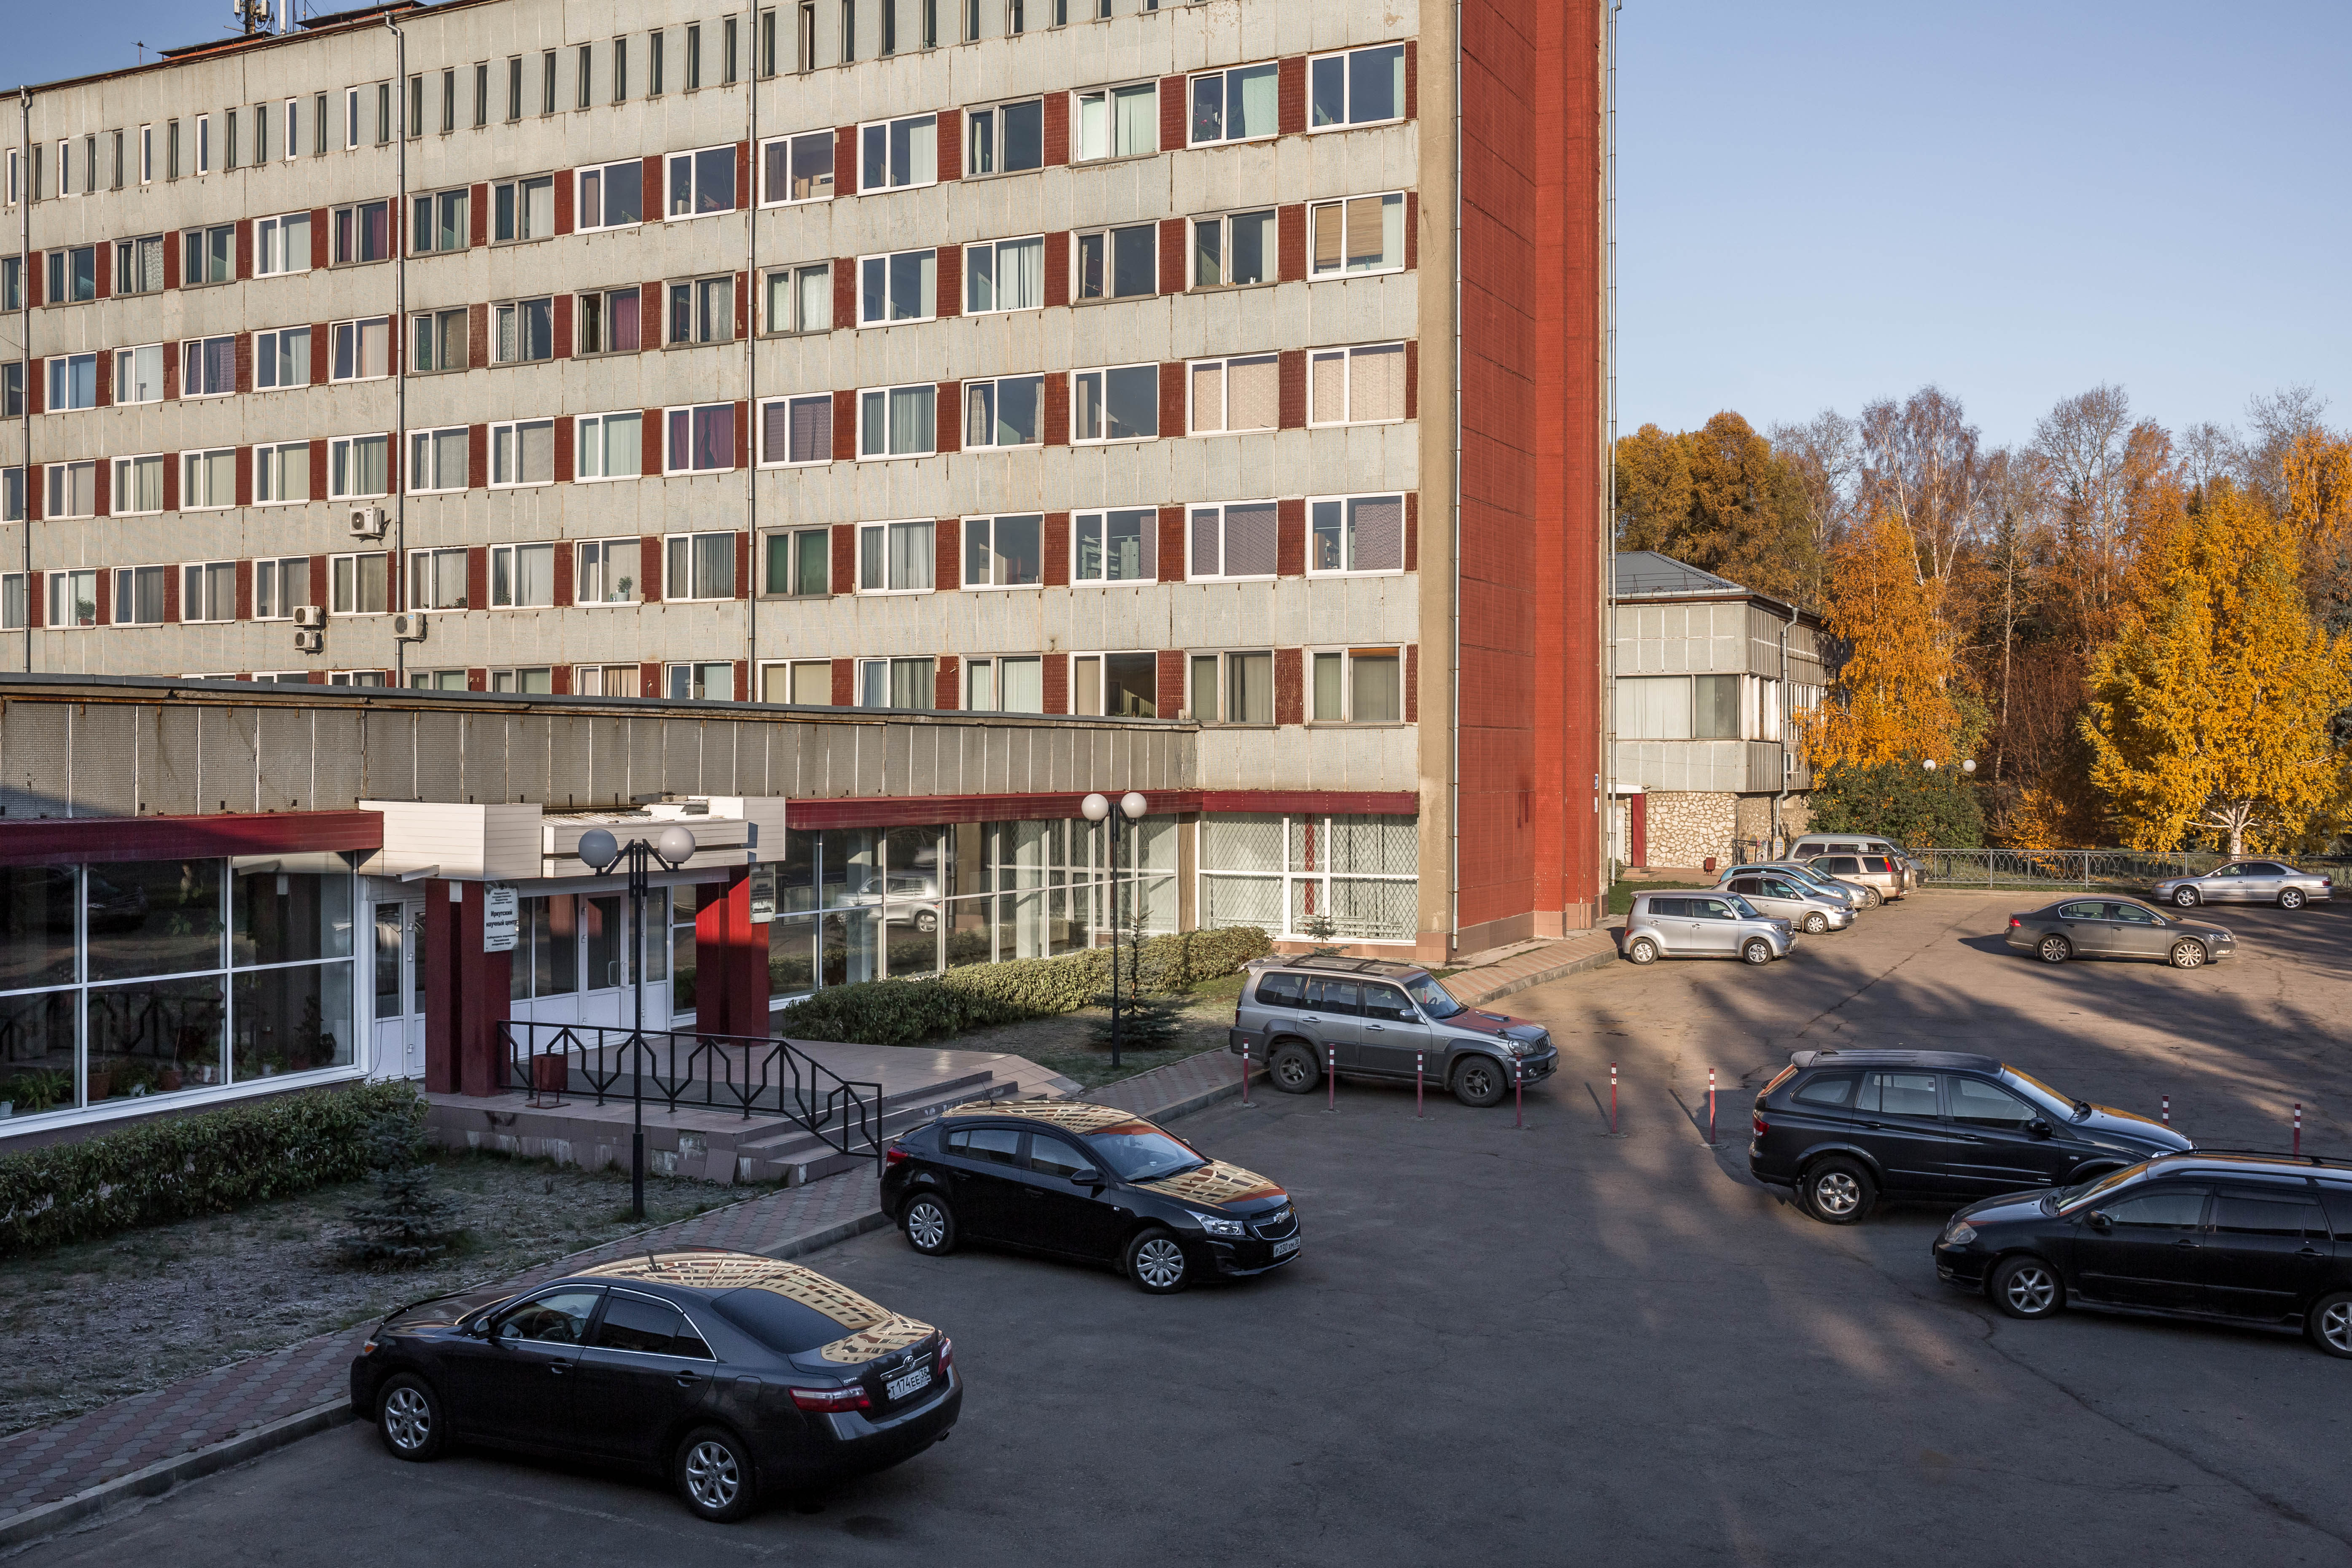
\includegraphics[width=0.7\linewidth]{institut.jpg}
  % \caption{1907 Родстер Франклина, Модель D. Фотография Harris \& Ewing, Inc. [Публичный доступ], размещено на Wikimedia Commons. (\url{https://goo.gl/VLCRBB}).}
  \caption{Фотография ИДСТУ СО РАН [Публичный доступ] (размещено на \url{idstu.irk.ru}) }
\end{figure}

Рисунки должны содержать подрисуночную подпись, представляющую читателю, что изображено. Подписи к рисункам находятся строго под рисунком. Рисунки также должны включать описание, подходящее для программ проговаривания текста, помогающим людям с ограниченными зрением знакомиться с вашей работой.  Подписи к рисункам располагаются под рисунком.

\section{Цитаты и ссылки на литературу}

Настоятельно рекомендуется использовать Bib\TeX{} для оформления ссылок на использованные источники. Имена авторов должны быть полными, используйте полные имена (<<Donald E. Knuth>>), а не инициалы (<<D. E. Knuth>>), в основные данные о публикации должны быть включены: название, год, том, номер, страницы, DOI статьи и т.~п.

Библиография входит в исходный документ обрамленной командами, расположенными непосредственно перед командой \verb|\end{document}|:
\begin{minted}{latex}
\bibliography{bibfile}
\end{minted}
Здесь <<\verb|bibfile|>> -- это имя Bib\TeX{}-файла без суффикса <<\verb|.bib|>>.

\subsection{Примеры}

Журнальная статья, разбитая на страницы -- \cite{Abril07}; журнальная статья с номером -- \cite{Cohen07}; ссылка на весь том -- \cite{JCohen96}, монография или книга -- \cite{Kosiur01}, монография иил книга в серии (см. 2a в спецификации  ) -- \cite{Harel79}, книга с выделенными частями, например антология или сборник, -- \cite{Editor00}; последующий пример оттуда же, указываем серию только в том случае, если указан номер тома \cite{Editor00a} (поэтому серия не должна присутствовать, так как у нее нет номера  тома); глава делимой -- \cite{Spector90}; глава книги в серии -- \cite{Douglass98}; многотомная работа в виде книги -- \cite{Knuth97}; статья в материалах конференции, симпозиума, практикума с разбивкой на страницы -- \cite{Andler79}; статья в материалах со всеми возможными элементами -- \cite{Smith10}; пример статьи с номером -- \cite{VanGundy07}, неофициально опубликованная работа -- \cite{Harel78}; диссертация -- \cite{Clarkson85}; магистерская диссертация -- \cite{anisi03}; онлайн-документ или веб-ресурс -- \cite{Thornburg01, Ablamowicz07, Poker06}; видеоигра (случай 1) -- \cite{Obama08} и (случай 2) -- \cite{Novak03} и \cite{Lee05}, (случай 3) патент -- \cite{JoeScientist001}; работа, принятая к публикации -- \cite{rous08}; плодовитый автор -- \cite{SaeediMEJ10} и \cite{SaeediJETC10}. Ссылки могут содержать <<дублирующие>> DOI- и URL-адреса, например, статьи SIAM \cite{Kirschmer:2010:AEI:1958016.1958018}. Многотомные работы в виде книг -- \cite{MR781536} и \cite{MR781537}. Пара цитирований с DOI: \cite{2004:ITE:1009386.1010128,Kirschmer:2010:AEI:1958016.1958018}. Онлайн-цитирования: \cite{TUGInstmem, Thornburg01, R, UMassCitations}.

\section{Благодарности}

Представление источников финансирования и другой поддержки, а также благодарность отдельным лицам и группам, которые помогали в исследовании и подготовке работы, должны быть включены в раздел благодарностей, который помещается непосредственно перед списком ссылок на использованные источники.  Этот раздел имеет особое окружение:
\begin{minted}{latex}
\begin{acknowledgments}
  Это разные виды разделов благодарности.
\end{acknowledgments}
\end{minted}
Предъявленные требования к оформлению позволяют информации, содержащуюся в этом разделе,  легко собирать на этапе извлечения метаданных, а также это обеспечивает корректность написания заголовков статей в содержании.  Не нужно оформлять этот раздел ни как пронумерованный или как ненумерованный {\verb|\section|}; пожалуйста, используйте только окружение <<{\verb|acknowgments|}>>.

\section{Приложения}

Если вашей статье требуется раздел"=приложение, добавьте его перед командой <<\verb|\end{document}|>> в конце исходного кода документа. Приложение начинается с команды <<\verb|appendix|>>:
\begin{minted}{latex}
\appendix
\end{minted}
Разделы в приложении пронумерованы буквами, а не цифрами.

%%
%% Секция благодарностей определяется средой "acknowledgments"
%% (НЕ при помощи непронумерованного раздела). Такой подход позволяет правильно
%% идентифицировать этот раздел в метаданных статьи, правильно
%% сформировать заголовок.

\begin{acknowledgments}
Благодарим разработчиков группы стилей LaTeX ACM \url{https://github.com/borisveytsman/acmart} и разработчиков из Elsevier, проведших улучшение шаблонов \LaTeX{} \url{https://www.ctan.org/tex-archive/macros/latex/contrib/els-cas-templates}.
\end{acknowledgments}

% Борьба с длиннющими URL-ы; предложено by Franck в
% https://tex.stackexchange.com/questions/636114/how-can-i-prevent-urls-in-an-eprint-field-from-overflowing-in-the-references-i/636172#636172
\Urlmuskip=0mu plus 1mu\relax

%%
%% Укажите файл библиографии
\bibliography{sample-ceur}

%%
%% Если надо раздел с приложением, то поместите его прямо после этой команды.
\appendix

\section{Онлайн-ресурсы}

Исходный код стиля ceur-art доступен по ссылке
\begin{itemize}
\item \href{https://github.com/yamadharma/ceurart}{GitHub},

% \item \href{https://www.overleaf.com/project/5e76702c4acae70001d3bc87}{Overleaf},
\item \href{https://www.overleaf.com/latex/templates/template-for-submissions-to-ceur-workshop-proceedings-ceur-ws-dot-org/pkfscdkgkhcq}{Шаблон Overleaf}.
\end{itemize}

\section{Онлайн-ресурсы 2}

\end{document}

%%
%% End of file
%%% Local Variables:
%%% mode: latex
%%% TeX-master: t
%%% End:
